\documentclass[twocolumn]{article}

\usepackage[letterpaper,margin=0.25in]{geometry}
\input{ncommon}
\everymath{}
\usepackage{titlesec}

\titleformat{\section}
  {\normalfont\fontsize{12}{15}\bfseries}{\thesection}{1em}{}
\titlespacing\section{0pt}{5pt plus 2pt minus 2pt}{3pt plus 2pt minus 2pt}
\titlespacing\subsection{0pt}{3pt plus 2pt minus 2pt}{3pt plus 2pt minus 2pt}
\titlespacing\subsubsection{0pt}{3pt plus 2pt minus 2pt}{3pt plus 2pt minus 2pt}
\renewcommand{\arraystretch}{1.5}

\title{ROB310 Midterm Aidsheet}
\author{Tyler Tian}

\begin{document}

\setlength{\abovedisplayskip}{3pt}
\setlength{\belowdisplayskip}{3pt}
\setlength{\parindent}{0pt}

\section{System Modelling}

Continuous time (linear):
$$\begin{aligned} \dot{\bm x}(t) &= \bm A\bm x(t) + \bm B\bm u(t), \bm x(0) = \bm x_0 \\ \bm y(t) &= \bm C\bm x(t) + \bm D\bm u(t)\end{aligned}$$
Continuous time (nonlinear):
$$\begin{aligned}\dot{\bm x}(t) &= \bm f(\bm x(t), \bm u(t)), \bm x(0) = \bm x_0 \\ \bm y(t) &= \bm h(\bm x(t), \bm u(t))\end{aligned}$$
Discrete time (linear):
$$\begin{aligned}\bm x_{k + 1} &= \bm A_d\bm x_k + \bm B_d\bm u_k \\ \bm y_k &= \bm C\bm x_k + \bm D\bm u_k\end{aligned}$$
With a zero-order hold:
\begin{gather*}\mattwo{\bm A_d}{\bm B_d}{\bm 0}{\bm I} = \exp\left(\mattwo{\bm A}{\bm B}{\bm 0}{\bm 0}h\right) \\
\bm A_d = e^{\bm Ah}, \bm B_d = \int _0^h e^{\bm A\tau'}\dd\tau'\bm B\end{gather*}

\section{Numerical Stability}

Well conditioned problem: $\operatorname{Cond}_x$ small or $\operatorname{cond}_x \leq 1$
\begin{gather*}
    \operatorname{Cond}_x = \abs*{\frac{\Delta\bar y}{\Delta x}} \approx \abs*{\diff{f}{x}} \\
    \operatorname{cond}_x = \abs*{\frac{\delta\bar y}{\delta x}} \approx \abs{K_x} = \abs*{\diff{f}{x} \cdot \frac{x}{f(x)}}
\end{gather*}
$\varphi$ is \textit{order} $p$ or $O(\Delta^p)$ if
$$\tilde y = \varphi(x, \Delta) - f(x) \propto \Delta^p$$
$\varphi$ is \textit{consistent} if
$$\lim _{\Delta \to 0} \varphi(x, \Delta) = f(x)$$
$\varphi$ is \textit{numerically stable} if
$$\abs*{\frac{\Delta\tilde y}{\Delta x}} \approx \abs*{\diff{\varphi}{x}} < 1$$
$\hat y = \varphi(\hat x, \Delta) = \varphi(\hat x + \Delta x)$ converges to $f(x)$ for $\Delta \to 0$ if it's consistent and at least marginally stable.

$\dot{\bm x} = \bm A\bm x$ well-conditioned/stable when $\Re(\lambda) < 0$ for all $\lambda$.

$\bm x_{k + 1} = \bm A\bm x$ well-conditioned/stable when $\abs{\lambda} < 1$ for all $\lambda$.

\section{Numerical Root Finding}

$f$ is \textit{Lipschitz continuous} if
$$\exists c\text{ s.t. }\forall x, z \in \reals, \abs{f(x) - f(z)} \leq c\abs{x - z}$$
An algorithm has \textit{convergence rate/order} $r$ if
$$\lim _{k \to \infty} \frac{\abs{E_{k + 1}}}{\abs{E_k}^r} = C$$

\textbf{Bisection}: order 1; requires continuity; have $l_k, r_k$ such that $\sgn f(l_k) \neq \sgn f(r_k)$, check $c = \frac{l_k + r_k}{2}$ each iteration.

\textbf{Fixed-point Iteration}: order 2 if $g'(x^*) \approx 0$, 1 otherwise; requires update function $g(x^*) = x^*$ for Lipschitz $g$ with $c < 1$ for $x \approx x^*$.
To find $g(x)$, rearrange $f(x^*) = 0$ into the form $x^* = g(x^*)$. Start with guess, update as $x_{k + 1} = g(x_k)$.

\textbf{Newton's Method}: order 2; requires continuous differentiability; equivalent to fixed-point iteration with $g(x) = x - \frac{f(x)}{f'(x)}$.
Start with guess, update as $x_{k + 1} = x_k - \frac{f(x_k)}{f'(x_k)}$. Exact for linear $f$ and suffers for highly nonlinear $f$.

\textbf{Secant Method}: order between 1 and 2; Newton's method, but use $f'(x_k) \approx \frac{f(x_k) - f(x_{k - 1})}{x_k - x_{k - 1}}$.

\section{Numerical Integration and Differentiation}

\textbf{Midpoint Rule}: order 2, approx. $f$ as constant between bounds
$$\int _{x_i}^{x_{i + 1}} f(x)\,\dx \approx (x_{i + 1} - x_i) \cdot f\left((x_{i + 1} + x_i)/2\right)$$

\textbf{Trapezoidal Rule}: order 2, approx. $f$ as linear
$$(x_{i + 1} - x_i) \cdot \frac{f(x_{i + 1}) + f(x_i)}{2}$$

\textbf{Simpson's Rule}: order 4, approx. $f$ as quadratic
$$(x_{i + 1} - x_i) \cdot \frac{f(x_{i + 1}) + 4f\left((x_{i + 1} + x_i)/2\right) + f(x_i)}{6}$$

\textbf{Forward Difference}: order 1
$$f'(x) \approx \frac{f(x + \Delta) - f(\Delta)}{\Delta}$$
\textbf{Backward Difference}: order 1
$$f'(x) \approx \frac{f(x) - f(x - \Delta)}{\Delta}$$
\textbf{Centered Difference}: order 2
$$f'(x) \approx \frac{f(x + \Delta) - f(x - \Delta)}{2\Delta}$$

\section{Numerical ODE Solving}

\textbf{Forward Euler's Method}: order 1 (global), 2 (local); explicit; conditionally stable if $\abs{1 + h\lambda} < 1$.
$$x_{k + 1} = x_k + hf_k$$

\textbf{Backward Euler's Method}: order 1 (global), 2 (local); implicit; conditionally stable if $\abs{1 - h\lambda} > 1$.
$$x_{k + 1} = x_k + hf_{k + 1}$$

\textbf{Trapezoidal Method}: order 2 (global), 3 (local); implicit; conditionally stable if $\abs*{\frac{1 + \frac{1}{2}h\lambda}{1 - \frac{1}{2}h\lambda}} < 1$.
$$x_{k + 1} = x_k + \frac{h}{2}(f_{k + 1} + f_k)$$

\textbf{Second-Order Runge-Kutta (Heun's Method, RK2)}: order 2 (global); explicit; conditionally stable if $-4 < 2h\lambda + h^2\lambda^2 < 0$.
$$x_{k + 1} = x_k + \frac{h}{2}\left(f(x_k + hf_k) + f_k\right)$$

\textbf{Fourth-Order Runge-Kutta (RK4)}: order 4 (global); explicit.
\begin{gather*}
    x_{k + 1} = x_k + \frac{h}{6}(k_1 + 2k_2 + 2k_3 + k_4) \\
    \begin{aligned}
        &k_1 = f(x_k), &k_2 = f\left(x_k + \frac{1}{2}hk_1\right) \\
        &k_3 = f\left(x_k + \frac{1}{2}hk_2\right), &k_4 = f(x_k + hk_3)
    \end{aligned}
\end{gather*}

\begin{center}
    \centering
    
\includegraphics[width=0.6\linewidth]{lec7_1.png}
    
\includegraphics[width=0.6\linewidth]{lec8_1.png}
\end{center}

\textit{Time constant}: for $\dot{\bm x} = \bm A\bm x$ with complex eigenvalues $\lambda _i$:
$$\tau _i = \Set{\frac{1}{\abs{\Re(\lambda _i)}}, \frac{2\pi}{\abs{\Im(\lambda _i)}}}$$
This ODE is \textit{stiff} if
$$\gamma = \frac{\tau _\text{max}}{\tau _\text{min}} > 10^3$$
Rule of thumb: simulate $T = 5\tau _\text{max}$ if system is stable; use step size $h = \min\Set{\frac{\tau _\text{min}}{10}, \frac{T}{200}}$ or number of steps $k = \max\Set{50\gamma, 200}$;
plot with step size $H = \frac{T}{200} = \frac{\tau _\text{max}}{40}$; for stiff systems use a variable-step solver with initial step $\frac{\tau _\text{min}}{10}$.
Use adaptive step size solvers for stiff problems.

\section{Optimization}

Formulation: minimize $f(\bm x)$, subject to $\bm g(\bm x) = \bm 0$ (equality constraints) and $\bm h(\bm x) \geq \bm 0$ (inequality constraints), where $f: \reals^n \mapsto \reals, \bm g: \reals^n \mapsto \reals^m, \bm h: \reals^n \mapsto \reals^p$.

$\bm x^*$ is a \textit{global minimum} if $$\forall \bm x \in \reals^n, f(\bm x^*) \leq f(\bm x)$$
$\bm x^*$ is a \textit{local minimum} if $$\exists \varepsilon > 0\text{ s.t. } \forall \bm x \in \reals^n, \norm{\bm x - \bm x^*}_2 < \varepsilon \implies f(\bm x^*) \leq f(\bm x)$$
All minima of $f$ are \textit{stationary points}, where $\del f(\bm x) = \bm 0$; to find the global minimum, check all stationary points and boundaries.

$$\bm H_f(\bm x) = \matthreeb{\ppdiff{f}{x_1}{x_1}}{\cdots}{\ppdiff{f}{x_1}{x_n}}{\vdots}{\ddots}{\vdots}{\ppdiff{f}{x_n}{x_1}}{\cdots}{\ppdiff{f}{x_n}{x_n}}$$
If $\bm x^*$ is a stationary point, it is a local minimum if $\bm H_f(\bm x^*) > 0$, maximum if $\bm H_f < 0$, saddle if $\bm H_f = 0$.

A \textit{feasible point} is any $\bm x$ satisfying all constraints; the \textit{feasible set} contains all feasible points.
A \textit{critical point} is a local maximum, minimum or saddle point in the feasible set.

\textit{Lagrange Multipliers}: for equality constraints $\bm g(\bm x) = \bm 0$:
$$\min _{\bm x, \bm\lambda}\Lambda(\bm x, \bm\lambda) = f(\bm x) - \bm\lambda^T\bm g(\bm x)$$

\textit{Karush-Kuhn-Tucker (KTT) Conditions}: $\bm x^*$ is a critical point when there exists $\bm\lambda \in \reals^m$ and $\bm\mu \in \reals^p$ such that:
\begin{enumerate}
    \itemsep 0pt
	\item Stationarity: $\del f(\bm x^*) - \sum _i \lambda _i\del g_i(\bm x^*) - \sum _j \mu _j\del h_j(\bm x^*) = \bm 0$
	\item Primal feasibility: $\bm g(\bm x^*) = \bm 0$ and $\bm h(\bm x^*) \geq \bm 0$
	\item Complementary slackness: $\forall j, \mu _jh_j(\bm x^*) = 0$
	\item Dual feasibility: $\forall j, \mu _j \geq 0$
\end{enumerate}

$f$ is \textit{convex} if $\bm H_f > 0$ for all $\bm x$, or
$$\forall \bm x_1 \neq \bm x_2, \forall \alpha \in (0, 1), f((1 - \alpha)\bm x_1 + \alpha\bm x_2) \leq (1 - \alpha)f(\bm x_1) + \alpha f(\bm x_2)$$
A set $S$ is \textit{convex} if:
$$\forall \bm x, \bm y \in S, \alpha \in [0, 1], \alpha\bm x + (1 - \alpha)\bm y \in S$$
If the objective $f$ and feasible set are both convex, the problem is convex and has a unique minimum.

\section{Numerical Optimization Algorithms}

$f$ is \textit{unimodular} over $[a, b]$ if there exists $x^* \in [a, b]$ s.t. $f$ is decreasing over $[a, x^*]$ and increasing over $[x^*, b]$.

\textbf{Golden Section Search}: 1D, unconstrained; order 1; requires unimodularity.
Rescale to $[0, 1]$, choose $x_0 = \alpha, x_1 = 1 - \alpha$ for $0 < \alpha < 1/2$; evaluate $f(x_0), f(x_1)$, discard larger side, rescale and repeat.
Using $1 - \alpha = \frac{1}{2}(\sqrt 5 - 1)$ allows using $x_0$ as the next $x_1$.
\begin{center}
    \centering
    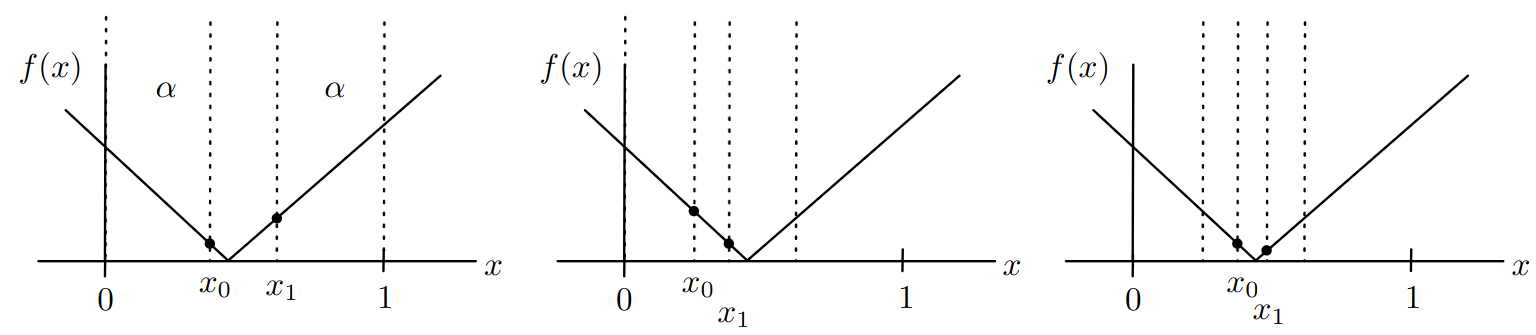
\includegraphics[width=\linewidth]{lec10_1.png}
\end{center}

\textbf{Gradient Descent}: unconstrained; requires twice differentiable.
Let $g(\alpha) = f(\bm x_k - \alpha\del f(\bm x_k)^T)$, find $\alpha^*$ minimizing $g$, update $x_{k + 1} = x_k - a^*\del f(\bm x_k)^T$.
Optimizing $g$ is expensive so fixed step size can be used. Suffers from poor conditioning of $f$.

\textbf{Newton's Method}: unconstrained; requires twice differentiable.
Iterate as $\bm x_{k + 1} = \bm x_k - \bm H_f^{-1}(\bm x_k)\del f(\bm x_k)^T$; or in 1D, $x_{k + 1} = x_k - \frac{f'(x_k)}{f''(x_k)}$.
Gauss-Newton approximates $\bm H_f$ using first derivatives (mix of gradient descent and Newton).
Levenberg-Marquardt applies adaptive regularization for nearly-singular Hessians.

\textbf{Sequential Quadratic Programming (SQP)}: constrained. Iteratively solves a series of simpler, less constrained approximations of the problem.
$f$ is replaced by a quadratic approximation and the constraints linearized. Similar to Newton's method; only converges if initial guess is good.

\textbf{Barrier Methods}: constrained. Constraints are turned into penalties on the objective.
Define new objective as $f'(x) = f(x) + \rho\frac{1}{h(x)}$ where weight $\rho$ is increased to satisfy constraints, decreased for more accuracy.

\section{Linear Algebra}

$\bm A^T\bm A$ is positive definite if $\bm A$ is full rank, semi-definite otherwise.

Orthogonal $\bm Q$ rotates, preserves angles, and $\bm Q^T\bm Q = \bm 1$.

$\bm A\bm x = \bm b$ can be solved by factoring $\bm A = \bm L\bm U$ and solving $\bm L\bm y = \bm b, \bm U\bm x = \bm y$.

A general \textit{vector norm} satisfies: $\norm{\bm x} = 0 \iff \bm x = \bm 0$; $\norm{c\bm x} = \abs{c}\norm{\bm x}$; $\norm{\bm x + \bm y} \leq \norm{\bm x} + \norm{\bm y}$.
The $p$\textit{-norm} for $p \geq 1$ is convex: $$\norm{\bm x}_p = (\abs{x_1}^p + \abs{x_2}^p + \cdots + \abs{x_n}^p)^{\frac{1}{p}}$$
2-norm is Euclidean; $\infty$-norm is $\norm{\bm x}_\infty = \max(\abs{x_1}, \abs{x_2}, \dots, \abs{x_n})$.

The \textit{matrix norm} induced by a vector norm is
$$\norm{\bm A} = \max\Set{\norm{\bm A\bm x} | \norm{\bm x} = 1} = \max _{\bm x \in \reals^n, \bm x \neq 0}\frac{\norm{\bm A\bm x}}{\norm{\bm x}}$$
\textit{1-norm}: maximum column sum
$$\norm{\bm A}_1 = \max_{i \leq j \leq n} \sum _{i = 1}^m \abs{a_{ij}}$$
\textit{2-norm}: largest eigenvalue of $\bm A$ (aka \textit{spectral radius})
$$\norm{\bm A}_2 = \max\Set{\sqrt{\lambda} | \exists\bm x \in \reals^n\text{ s.t. }\bm A^T\bm A\bm x = \lambda\bm x}$$
\textit{Frobenius norm}: always $\norm{\bm A}_2 \leq \norm{\bm A}_F$
$$\norm{\bm A}_F = \sqrt{\sum _{i = 1}^m\sum _{j = 1}^n \abs{a_{ij}}^2} = \sqrt{\tr \bm A^T\bm A}$$
$\infty$\textit{-norm}: maximum row sum
$$\norm{\bm A}_\infty = \max _{1 \leq i \leq m} \sum _{j = 1}^n \abs{a_{ij}}$$

The \textit{condition number} of $\bm A$ with respect to a norm is
$$\operatorname{cond} \bm A = \norm{\bm A}\norm{\bm A^{-1}}$$
or $\infty$ if $\bm A$ is non-invertible.
For solving $\bm A\bm x = \bm b$, this describes how error in $\bm A$ and $\bm b$ propagates to $\bm x$.

\end{document}
